% =====================================================================
%  Figura: mecanismo del exoesqueleto (modelo simplificado) montado
%  sobre un dedo simbolico.
%
%  - El diagrama de eslabones se replica con TikZ (una sola fuente de
%    verdad, vectorial y editable).
%  - Con \confondotrue se incluye la foto del dedo (fondo eliminado)
%    como capa de fondo y el mecanismo se dibuja encima de las falanges.
%  - Con \confondofalse se compila SOLO el diagrama (util para validar).
%
%  Compilar:  pdflatex exo_sobre_dedo.tex
% =====================================================================
\documentclass[border=6pt]{standalone}
\usepackage{tikz}
\usepackage{amsmath}
\usetikzlibrary{arrows.meta,calc,decorations.pathreplacing}

% ---- Interruptor: incluir la foto del dedo como fondo -----------------
\newif\ifconfondo
\confondotrue             % \confondotrue = con foto del dedo ; \confondofalse = solo diagrama

% ---- Nombre del archivo de la foto (dedo sin fondo, PNG con alfa) -----
\newcommand{\dedoimg}{dedo_sin_fondo.png}

% ---- Parametros de montaje de la foto (se ajustan al calibrar) --------
% Con x=y=0.62cm, el ancho en cm = (unidades deseadas) * 0.62.
\newcommand{\dedoancho}{18.6cm}   % ~30 unidades de ancho
\newcommand{\dedox}{14.1}         % centro X de la foto (coords del dibujo)
\newcommand{\dedoy}{2.7}          % centro Y de la foto (coords del dibujo)

% =====================================================================
\begin{document}
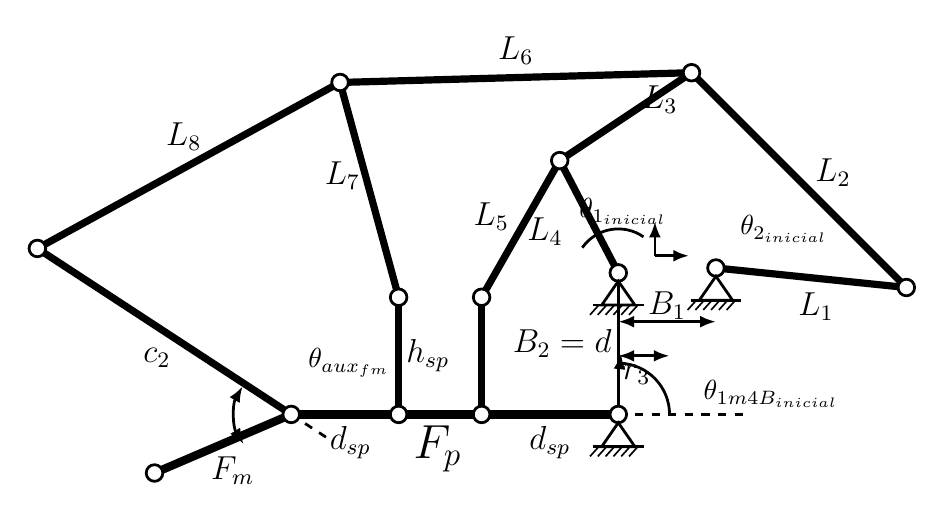
\begin{tikzpicture}[
    x=0.62cm,y=0.62cm,
    esl/.style={line width=2.6pt,line cap=round,black},   % eslabon
    fal/.style={line width=3.0pt,line cap=round,black},    % falange
    cota/.style={line width=1.0pt,{Latex[length=2mm]}-{Latex[length=2mm]}},
    dbl/.style={line width=1.0pt,{Latex[length=2mm]}-{Latex[length=2mm]}},
    ref/.style={line width=1.0pt,dashed},
    ejeflecha/.style={line width=1.0pt,-{Latex[length=2mm]}},
  ]

  % -------------------------------------------------------------------
  % (0) Capa de fondo: foto del dedo (opcional)
  % -------------------------------------------------------------------
  \ifconfondo
    \node[anchor=center,inner sep=0pt] at (\dedox,\dedoy)
      {\includegraphics[width=\dedoancho]{\dedoimg}};
  \fi

  % -------------------------------------------------------------------
  % (1) Coordenadas de los nodos  (x derecha, y arriba)
  %     Reproducen el diagrama simplificado proporcionado.
  % -------------------------------------------------------------------
  \coordinate (A)  at (1.8, 7.2);    % junta far-left  (L8, c2)
  \coordinate (B)  at (8.0,10.6);    % sup-izq         (L6, L7, L8)
  \coordinate (C)  at (15.2,10.8);   % sup-der         (L6, L2, L3)
  \coordinate (D)  at (19.6, 6.4);   % extremo der     (L1, L2)
  \coordinate (E)  at (12.5, 9.0);   % central         (L3, L4, L5)
  \coordinate (F)  at (13.7, 6.7);   % pivote tierra izq (theta1, L4)
  \coordinate (G)  at (15.7, 6.8);   % pivote tierra der (theta2, L1)
  \coordinate (H)  at (9.2, 6.2);    % base de L7
  \coordinate (Hf) at (9.2, 3.8);    % pie de h_sp
  \coordinate (I)  at (10.9, 6.2);   % base de L5
  \coordinate (If) at (10.9, 3.8);   % pie de L5
  \coordinate (K)  at (7.0, 3.8);    % vertice theta_aux_fm (Fp-Fm-c2)
  \coordinate (M)  at (13.7, 3.8);   % pivote tierra inf (theta_1m4B)
  \coordinate (Fmp) at (4.2, 2.6);   % extremo libre de Fm

  % -------------------------------------------------------------------
  % (2) Eslabones de la cadena
  % -------------------------------------------------------------------
  \draw[esl] (G) -- (D);   % L1
  \draw[esl] (D) -- (C);   % L2
  \draw[esl] (C) -- (E);   % L3
  \draw[esl] (E) -- (F);   % L4
  \draw[esl] (E) -- (I);   % L5
  \draw[esl] (B) -- (C);   % L6
  \draw[esl] (B) -- (H);   % L7
  \draw[esl] (A) -- (B);   % L8
  \draw[esl] (H) -- (Hf);  % vertical h_sp
  \draw[esl] (I) -- (If);  % vertical (pie de L5)
  \draw[esl] (A) -- (K);   % c2
  \draw[fal] (K) -- (M);   % falange proximal Fp
  \draw[fal] (K) -- (Fmp); % falange medial Fm

  % Bancada B2=d : linea vertical fina entre F y M
  \draw[line width=1pt] (F) -- (M);

  % -------------------------------------------------------------------
  % (3) Lineas de referencia punteadas (angulos auxiliares)
  % -------------------------------------------------------------------
  % prolongacion de c2 (A->K) para theta_aux_fm (corta, para no cruzar F_p)
  \draw[ref] (K) -- ($ (A)!1.14!(K) $);
  % referencia horizontal en M para theta_1m4B
  \draw[ref] (M) -- ++(2.6,0);

  % -------------------------------------------------------------------
  % (4) Juntas (circulos blancos)
  % -------------------------------------------------------------------
  \foreach \n in {A,B,C,D,E,F,G,H,I,K,M,Fmp,Hf,If}{
    \filldraw[fill=white,draw=black,line width=1pt] (\n) circle (0.17);
  }

  % -------------------------------------------------------------------
  % (5) Bancadas (triangulo + rayado) en F, G, M
  % -------------------------------------------------------------------
  \foreach \n in {F,G,M}{
    \begin{scope}[shift={(\n)}]
      \draw[line width=1pt] (0,-0.17) -- (-0.34,-0.66) -- (0.34,-0.66) -- cycle;
      \draw[line width=1pt] (-0.52,-0.66) -- (0.52,-0.66);
      \foreach \x in {-0.40,-0.24,-0.08,0.08,0.24,0.40}{
        \draw[line width=0.6pt] (\x,-0.66) -- (\x-0.18,-0.86);
      }
    \end{scope}
  }

  % -------------------------------------------------------------------
  % (6) Etiquetas de eslabones
  % -------------------------------------------------------------------
  \tikzset{lab/.style={font=\itshape\large}}
  \node[lab] at ($ (G)!0.5!(D) + (0.1,-0.6) $) {$L_1$};
  \node[lab] at ($ (D)!0.5!(C) + (0.7,0.15) $) {$L_2$};
  \node[lab] at ($ (C)!0.5!(E) + (0.7,0.35) $) {$L_3$};
  \node[lab] at ($ (B)!0.5!(C) + (0,0.55) $)   {$L_6$};
  \node[lab] at ($ (A)!0.5!(B) + (-0.1,0.6) $) {$L_8$};
  \node[lab] at ($ (B)!0.5!(H) + (-0.55,0.3) $){$L_7$};
  \node[lab] at ($ (E)!0.5!(I) + (-0.6,0.25) $){$L_5$};
  \node[lab] at ($ (E) + (-0.30,-1.45) $)      {$L_4$};
  \node[lab] at ($ (A)!0.5!(K) + (-0.15,-0.55) $){$c_2$};
  \node[lab] at ($ (K)!0.5!(Fmp) + (0.2,-0.55) $){$F_m$};

  % Fp y d_sp sobre la falange proximal
  \node[lab] at ($ (K)!0.55!(Hf) + (0,-0.58) $) {$d_{sp}$};
  \node[lab] at ($ (If)!0.5!(M) + (0,-0.58) $) {$d_{sp}$};
  \node[lab] at ($ (Hf)!0.5!(If) + (-0.05,-0.7) $) {\itshape\LARGE $F_p$};

  % h_sp junto a la vertical de L7
  \node[lab] at ($ (H)!0.5!(Hf) + (0.6,0) $) {$h_{sp}$};

  % B2 = d (cota vertical, a la izquierda de la linea F-M)
  \node[lab] at ($ (F)!0.5!(M) + (-1.15,0) $) {$B_2=d$};

  % -------------------------------------------------------------------
  % (7) Cotas horizontales B1 y r3 (entre pivotes a tierra)
  % -------------------------------------------------------------------
  \coordinate (b1a) at ($ (F) + (0,-1.0) $);
  \coordinate (b1b) at (15.7,5.7);
  \draw[cota] (b1a) -- (b1b);
  \node[lab] at ($ (b1a)!0.5!(b1b) + (0,0.32) $) {$B_1$};

  \coordinate (r3a) at ($ (F) + (0,-1.7) $);
  \coordinate (r3b) at ($ (r3a) + (1.05,0) $);
  \draw[cota] (r3a) -- (r3b);
  \node[lab] at ($ (r3a)!0.5!(r3b) + (-0.15,-0.38) $) {$r_3$};

  % -------------------------------------------------------------------
  % (8) Angulos de entrada y marco de referencia local
  % -------------------------------------------------------------------
  % theta_1_inicial en F (arco + flecha)
  \draw[line width=1pt] ($ (F) + (0.75:0) $) ++(55:0.9) arc (55:145:0.9);
  \node[lab,font=\itshape\normalsize] at ($ (F) + (0.1,1.25) $) {$\theta_{1_{inicial}}$};
  % marco de referencia local (x,y) junto a theta_1
  \draw[ejeflecha] ($ (F)+(0.75,0.35) $) -- ++(0,0.7);
  \draw[ejeflecha] ($ (F)+(0.75,0.35) $) -- ++(0.7,0);

  % theta_2_inicial en G
  \node[lab,font=\itshape\normalsize,anchor=west] at ($ (G) + (0.3,0.8) $) {$\theta_{2_{inicial}}$};

  % theta_1m4B_inicial en M (arco desde la horizontal punteada hacia F)
  \draw[line width=1pt] ($ (M) + (0:1.05) $) arc (0:88:1.05);
  \draw[ejeflecha] ($ (M) + (88:1.05) $) -- ++(0.02,0.2);
  \node[lab,font=\itshape\normalsize,anchor=west] at ($ (M) + (1.55,0.42) $) {$\theta_{1m4B_{inicial}}$};

  % theta_aux_fm en K (arco de doble punta entre ref c2 y Fm)
  \draw[dbl] ($ (K) + (150:1.15) $) arc (150:212:1.15);
  \node[lab,font=\itshape\normalsize,anchor=west] at ($ (K) + (0.15,1.05) $) {$\theta_{aux_{fm}}$};

\end{tikzpicture}
\end{document}
